\documentclass[10pt,twocolumn]{article}
\usepackage[margin=0.68in]{geometry}
\usepackage{amsmath,amssymb,booktabs,graphicx,microtype,url,xcolor}
\usepackage[hidelinks]{hyperref}
\setlength{\columnsep}{0.24in}
\title{GeoBEACON: Joint Semantic, Streaming, and Lighting Budget Control\\
for a Vulkan Urban Digital Twin}
\author{Swayam Singal}
\date{July 2026}

\begin{document}
\maketitle

\begin{abstract}
Urban digital twins must distribute finite frame time, graphics memory, and upload bandwidth across
geometry detail and lighting accuracy. Fixed level of detail (LOD) and distance-only selection
ignore the task relevance of landmarks, intersections, and route corridors; lighting-only
adaptation ignores the cost of making city geometry resident. This paper presents GeoBEACON, a
reproducible Vulkan research renderer over a checked OpenStreetMap (OSM) extract of Connaught Place,
New Delhi. GeoBEACON combines semantic tile utility, asynchronous three-level geometry streaming,
camera-space clustered lighting, aggregate-bounded diffuse-light pruning, temporal hysteresis, and a
10 Hz budget controller. The artifact includes deterministic OSM preprocessing to glTF 2.0 and 3D
Tiles 1.1, five recorded camera paths, dual-driver measurement classes, exact diffuse captures, raw
frame CSVs, and figure regeneration. A 20-case dual-driver pilot completed without failures. On
MoltenVK, bounded GeoBEACON reduced median measured cluster-plus-lighting GPU time from 0.2602 ms for
fixed LOD1/fixed clusters to 0.1308 ms in this 100-light validation workload; the result is reported
as artifact evidence rather than a general performance claim.
\end{abstract}

\section{Introduction}
An urban renderer has coupled resource decisions. Selecting a detailed facade increases vertex and
index traffic, resident memory, upload work, visible primitives, and potentially the number of
fragments that traverse local light lists. Conversely, aggressive geometry simplification can erase
the landmarks and intersections that make a digital twin useful even when conventional image error
is small. A controller that treats geometry, streaming, and lighting as independent subsystems can
therefore satisfy each local budget while making a poor global allocation.

GeoBEACON tests the following hypothesis:
\begin{quote}
\emph{Joint semantic and view-aware allocation of geometry detail, streaming bandwidth, memory, and
lighting accuracy provides greater perceptual and task-relevant utility per millisecond than fixed
LOD, distance-only LOD, or lighting-only adaptation.}
\end{quote}
The contribution is the unified and ablatable allocation system, not SSBOs, clustered shading,
instancing, glTF, 3D Tiles, or bounded light selection individually. The implementation retains the
original BEACON techniques as regression baselines and adds five city policies: fixed LOD1,
distance LOD, semantic LOD, GeoBEACON exact, and GeoBEACON bounded.

The artifact makes three distinctions that are essential for credible systems research. First,
conservative omitted-light bounds and measured image error are separate quantities. Second, Vulkan
GPU timestamps, Vulkan CPU fallback timings, and analytical predictions occupy separate result
classes. Third, adaptation mode includes controller settling, while steady-state experiments can
freeze parameters after warm-up.

\clearpage
\section{Prior Work and Positioning}
Tiled and clustered shading established spatially restricted light lists as a practical forward
many-light technique. Lightcuts and later virtual-point-light methods established bounded
approximation, while grid-based reservoirs such as ReGIR combine spatial grids with stochastic
reuse for much larger light populations~\cite{vpl,regir}. GeoBEACON remains deterministic and
targets finite-radius direct point lights. Neural visibility caches introduce online learning and
inference behavior outside this study's reproducibility constraints~\cite{nvc}.

Geospatial runtimes commonly use hierarchical tiles, screen-space error, and progressive content.
OGC 3D Tiles 1.1 standardizes a spatial hierarchy over renderable tile payloads~\cite{tiles}. OSM
provides open vector geometry and semantic tags under the ODbL~\cite{osm}. GeoBEACON connects these
standards-oriented data structures to a renderer-level joint controller and exposes semantic
weighting as a dedicated ablation.

\section{Canonical Dataset}
The study area is Connaught Place, New Delhi, bounded by latitude $28.6270$--$28.6365$ and longitude
$77.2070$--$77.2245$. The repository commits the canonical OSM 0.6 XML extract so building and
benchmark execution do not depend on network availability. The source SHA-256 is recorded in every
derived manifest. Network acquisition is an explicit offline action with one-request concurrency,
identifying user agent, cache, size limit, timeout, and exponential backoff.

The deterministic preprocessor parses nodes, ways, and multipolygon relations; rejects malformed
features; converts WGS84 coordinates to a double-precision local east-north frame; and partitions
features into 128 m cells. Height precedence is explicit:
\[
h=\begin{cases}
\texttt{height},&\text{when valid},\\
3.2\,\texttt{building:levels},&\text{otherwise},\\
h_{\mathrm{class}},&\text{otherwise}.
\end{cases}
\]
Minimum levels, bridges, tunnels, and layer tags influence vertical placement. Roads become
class- and lane-aware ribbons. Materials use deterministic colors rather than downloaded imagery.
The checked output contains 151 spatial records and 453 GLBs across LOD0, LOD1, and LOD2. Every GLB
is reloaded before acceptance, and the report records vertex/index counts, invalid inputs, semantic
counts, bounds, checksums, attribution, and license.

LOD0 contains tile ground, urban proxies, and major roads. LOD1 contains extruded footprints, roads,
water, vegetation, and semantic colors. LOD2 retains individual features and minor roads. The
runtime manifest accompanies an OGC-style 3D Tiles 1.1 \texttt{tileset.json}. Engine code remains
MIT licensed; source and derived OSM data carry separate ODbL notices. The rendered window includes
``© OpenStreetMap contributors''.

\clearpage
\section{Streaming Runtime}
The geospatial runtime is independent of the tutorial's object map. Each tile progresses through
\texttt{Unloaded}, \texttt{Queued}, CPU loading, upload waiting, \texttt{Resident}, eviction, or
\texttt{Failed}. Worker threads perform file I/O and GLB decoding only. Vulkan model creation occurs
on the render thread, preserving device ownership. A generation counter cancels stale requests when
the desired LOD changes before upload.

At 10 Hz, the selector performs double-precision bounds tests and ranks visible candidates. For a
tile $t$ and representation $r$, utility is
\begin{equation}
U(t,r)=w_s(t)A_{\rm screen}(t)V(t)Q(r)S_{\rm temporal}(t),
\end{equation}
and cost is
\begin{equation}
C(t,r)=C_{\rm gpu}(t,r)+\lambda_mM(t,r)+\lambda_bB(t,r)+\lambda_lL(t,r).
\end{equation}
Here $w_s$ is semantic importance, $A_{\rm screen}$ is projected importance, $V$ is visibility
confidence, $Q$ is representation quality, $S_{\rm temporal}$ rewards stability, $M$ is memory,
$B$ is upload demand, and $L$ estimates lighting work. Candidates are ordered by marginal utility
per byte for deterministic selection.

Visible landmarks, primary roads, intersections, and route-adjacent content receive larger
importance. Fixed LOD1 disables semantic differentiation; distance LOD removes $w_s$; semantic LOD
uses $w_s$ without lighting control. GeoBEACON exact and bounded use the joint policy. Representation
downgrades require 30 controller ticks of lifetime, and at most eight tile changes enter a frame.
Separate upgrade/downgrade pressure prevents oscillation.

Upload bandwidth is enforced by a token bucket. Cold-cache runs begin with no resident models;
warm-cache runs bypass bandwidth throttling during the warm-up residency phase. Resident bytes are
recomputed from actual representation files. Budget-aware LRU eviction excludes visible tiles and
moves resources into a deferred retirement queue. Retirement occurs only after more frames than the
maximum frames in flight and a device-idle synchronization before destruction, preventing
in-flight resource release. Failed content remains a recorded diagnostic state rather than
silently disappearing.

The runtime reports visible, requested, resident, upgraded, downgraded, and failed tiles; bytes
resident and uploaded; p95 request latency; representation churn; semantic utility; and budget
violations. These are frame-level values, not only end-of-run aggregates.

\clearpage
\section{Camera-Space Lighting}
The exact diffuse reference stores an unrestricted light array in an SSBO and evaluates all active
finite-radius point lights. The visual forward baseline retains specular shading but is excluded
from formal error comparisons. A light's diffuse contribution uses finite-radius attenuation and
inverse squared distance.

The fixed GPU builder uses a $16\times9\times24$ camera-space grid. XY membership comes from the
projected light sphere, while logarithmic depth is
\begin{equation}
z_{\rm slice}=\left\lfloor N_z
\frac{\log(z/z_n)}{\log(z_f/z_n)}\right\rfloor .
\end{equation}
Assignment consists of five compute stages:
\begin{enumerate}
  \item clear headers, cursors, and block sums;
  \item dispatch one invocation per light and atomically count its cluster range;
  \item perform 256-element block exclusive scans and scan block sums;
  \item add block offsets and record overflow;
  \item scatter light IDs into compact contiguous storage.
\end{enumerate}
Compute barriers establish count-to-scan, scan-to-offset, offset-to-scatter, and
scatter-to-fragment visibility. Timestamp labels isolate count, local scan, block scan, offset, and
scatter intervals.

No overflow is silently truncated. A header whose candidate count exceeds its list cap, or whose
offset would exceed storage, sets an overflow flag. The fragment shader then evaluates all global
lights for that cluster, which is slower but exact because finite-radius attenuation rejects
non-influential lights.

\subsection{Adaptive bounded evaluation}
Adaptive BEACON starts with coarse XY tiles and chooses 1, 2, 4, or 8 depth leaves. Exact mode keeps
all intersecting lights. For bounded mode, light $l$ and cluster $c$ receive the diffuse bound
\begin{equation}
E_{\max}(l,c)\le
\frac{I_l\rho_{\max}}{\max(d_{\min}(l,c)^2,\epsilon_d)}.
\end{equation}
Candidates are sorted or bucketed from weakest to strongest. Removal stops before the aggregate
omitted bound exceeds $\varepsilon_c$:
\begin{equation}
\sum_{l\in R(c)}E_{\max}(l,c)\le\varepsilon_c.
\end{equation}
This prevents many individually weak lights from collectively violating quality. Sparse clusters
store explicit 32-bit indices. Dense clusters store bitsets. Bitset traversal is word-wise:
\texttt{findLSB} selects a set bit and \texttt{word \&= word-1} clears it, so shader work scales with
retained lights rather than the global light population.

\clearpage
\section{Joint Budget Controller}
The controller receives target frame milliseconds, memory bytes, upload MiB/s, global diffuse error,
and a maximum tile-change rate. Measured cluster-build, lighting, upload, and total-frame values
enter exponentially weighted moving averages. Scheduling occurs at 10 Hz rather than every frame.
This separates resource decisions from frame noise and reduces list and residency churn.

Geometry and lighting share priorities. Landmark, intersection, primary-road, and near-facade tiles
receive tighter local light-error allowances. Distant and low-importance tiles receive looser
allowances, but the controller never exceeds the global sum of omitted bounds. When total frame time
exceeds the high threshold, the controller reduces changes and subdivision pressure. When time
remains below the low threshold, it cautiously improves quality. The split and merge thresholds are
different, and minimum lifetimes prevent threshold chatter.

The controller exposes its decisions through counters rather than hiding them in a black box:
subdivision depth, active clusters, explicit/bitset distribution, retained and pruned samples,
predicted bound, split/merge count, cluster churn, visible/resident tiles, LOD churn, uploads, memory,
and budget violations. This transparency supports ablation and replay.

\section{Experimental Protocol}
Five deterministic camera paths target different failure modes: outer orbit tests broad visibility;
street drive tests continuity; intersection dwell emphasizes semantic hotspots; landmark approach
tests progressive quality; and rapid teleport stresses cancellation, upload, and eviction. Benchmark
frames use a fixed $1/60$ s timestep and recorded transforms.

The full matrix spans 100, 500, and 2,000 lights; 16.67 and 33.33 ms frame budgets; 256, 512, and
1,024 MiB memory; 25, 100, and effectively unlimited MiB/s upload; 720p, 1080p, and 1440p; cold and
warm caches; MoltenVK and KosmicKrisp; and five repeated trials. Each full case warms for 600 frames
and measures 1,800 frames.

Every run records the git commit, shader hashes, device identity and UUID, Vulkan API and driver,
capabilities, policy, path, random seed, resolution, cache mode, source checksum, budgets, and
measurement class. GPU-query rows are never merged with CPU fallback or analytical predictions.
The exact reference uses maximum resident geometry for its selected frame, exact diffuse SSBO
lighting, identical camera/light state and exposure, and no light pruning.

\clearpage
\section{Pilot Results}
The checked pilot is an instrumentation validation: 20 cases, all five policies, two routes, both
local ICDs, 100 lights, 640$\times$360, 256 MiB, 25 MiB/s, cold cache, 30 warm-up frames, and 60
measured frames. All 20 completed. It is intentionally reported separately from the full
five-repeat matrix.

\begin{table}[h]
\centering
\small
\caption{Pilot medians and p95 CPU frame time. GPU is cluster build plus lighting.}
\begin{tabular}{llrrr}
\toprule
Driver & Policy & CPU50 & CPU95 & GPU50\\
 & & ms & ms & ms\\
\midrule
MoltenVK & Fixed LOD1 & 7.221 & 8.709 & 0.2602\\
MoltenVK & Geo exact & 8.331 & 12.156 & 0.1875\\
MoltenVK & Geo bounded & 8.270 & 12.364 & 0.1308\\
KosmicKrisp & Fixed LOD1 & 8.353 & 12.060 & --\\
KosmicKrisp & Geo exact & 13.147 & 17.891 & --\\
KosmicKrisp & Geo bounded & 12.914 & 18.185 & --\\
\bottomrule
\end{tabular}
\end{table}

\begin{figure}[h]
\centering
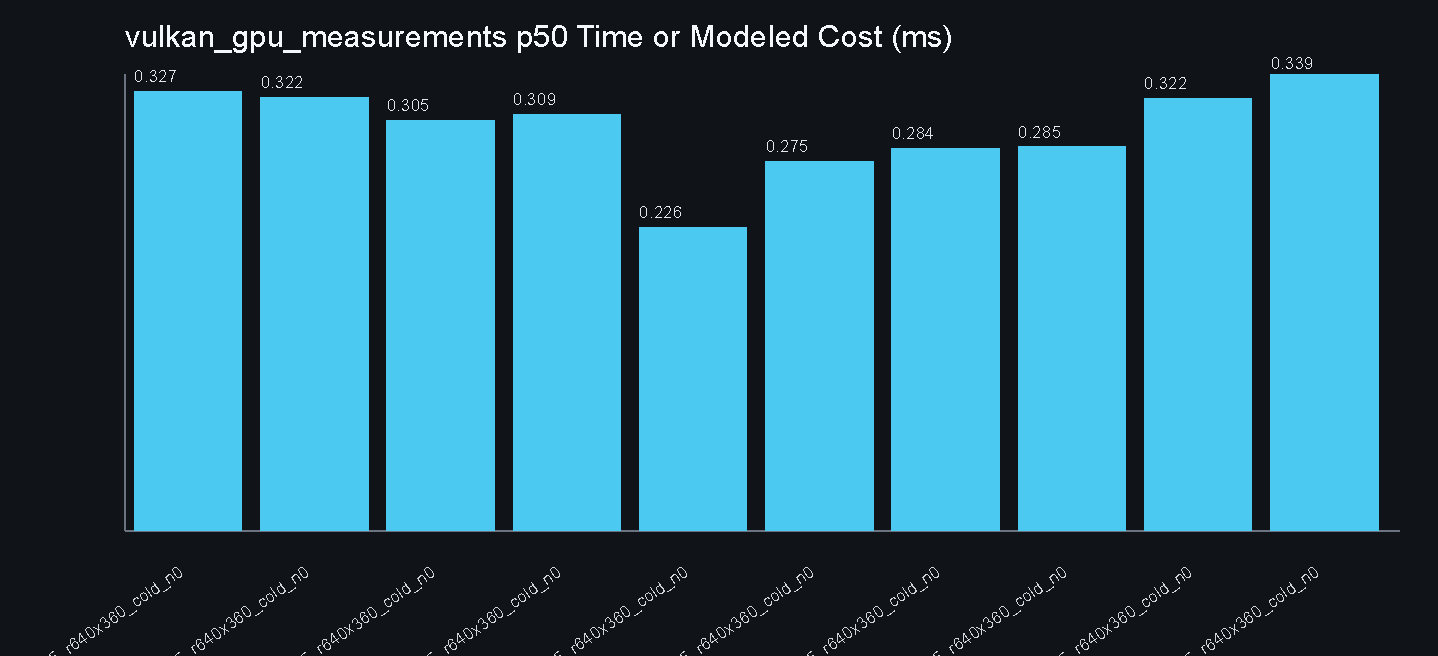
\includegraphics[width=\columnwidth]{geobeacon_gpu_p50.pdf}
\caption{MoltenVK timestamp-query pilot values generated from raw frame CSVs.}
\end{figure}

\begin{figure}[h]
\centering
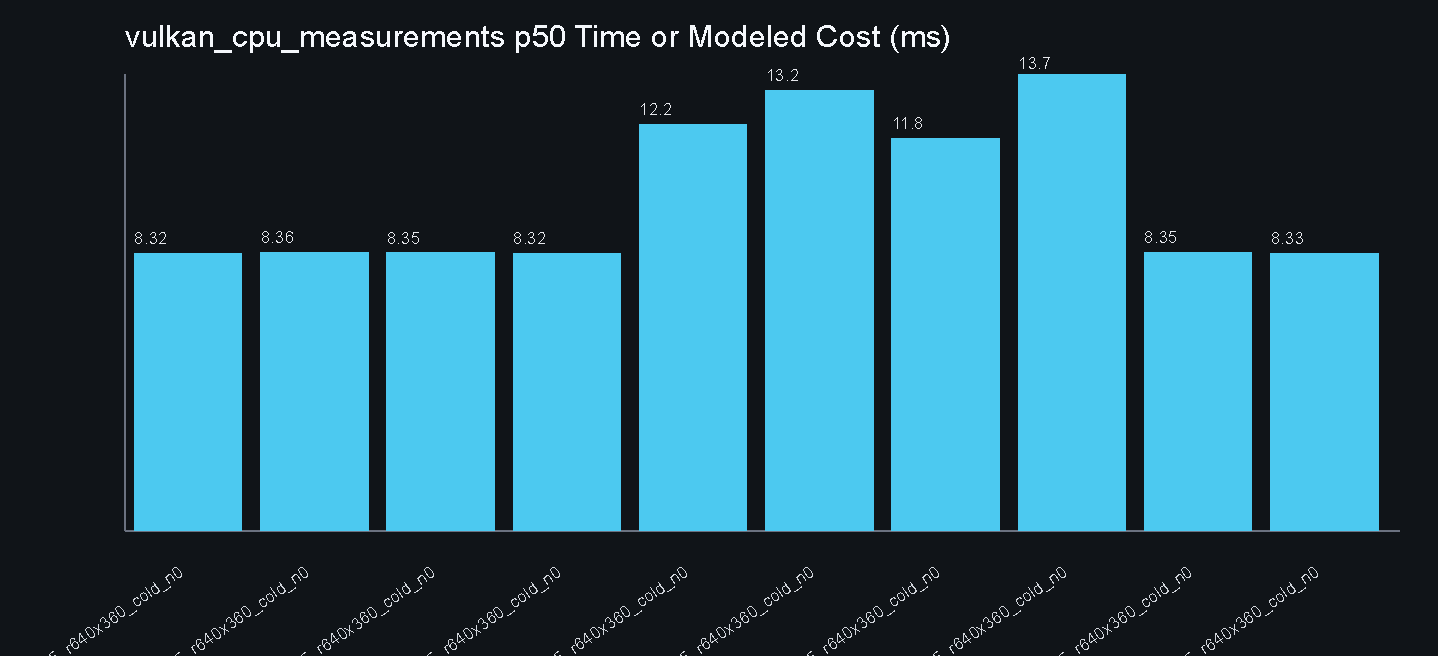
\includegraphics[width=\columnwidth]{geobeacon_cpu_p50.pdf}
\caption{KosmicKrisp CPU-fallback pilot values; no GPU time is inferred.}
\end{figure}

MoltenVK reported timestamp queries; KosmicKrisp did not. The bounded policy's lower GPU median in
this workload is consistent with fewer evaluated light samples, but the pilot is too small for a
cross-scene causal claim. CPU p95 increased for adaptive policies because CPU hierarchy construction
and exact capture synchronization remain visible in the validation configuration. This negative
result is retained.

Exact and bounded capture pairs reported MSE separately from conservative bounds. The saved PPM
captures verify that the compared buffers contain rendered city geometry rather than only a clear
color. Bounded pilot MSE was zero at RGBA8 quantization on most cases and $2.26\times10^{-11}$ on
KosmicKrisp in aggregate; this does not prove the analytical bound, but confirms the image-measurement
path and motivates higher-light full runs.

\clearpage
\section{Verification and Reproduction}
CTest covers contribution bounds, encoding selection, controller response, exclusive scan offsets,
capacity overflow, coordinate conversion, height precedence, polygon orientation, source checksum,
and reload of all 453 committed GLBs. Release builds compile vertex, fragment, and compute shaders
as executable dependencies. Physical-device selection accepts index, UUID, or name substring.
Instance creation negotiates Vulkan 1.2 against the loader and enables portability enumeration when
available.

Both local ICD manifests execute:
\begin{itemize}
\item \texttt{/usr/local/share/vulkan/icd.d/MoltenVK\_icd.json};
\item \texttt{/usr/local/share/vulkan/icd.d/libkosmickrisp\_icd.json}.
\end{itemize}
The matrix runner is resumable: a case with an existing frame CSV is treated as cached unless
\texttt{--force} is supplied. It writes a matrix manifest including failures and elapsed time.
The figure script uses only the Python standard library and regenerates SVG plots and a Markdown
summary from raw rows.

Correctness invariants are explicit. Exact modes retain every intersecting light. A list overflow
selects the exact fallback. Worker threads never call Vulkan. Stale loads are discarded by
generation. Resident resources enter deferred retirement and are synchronized before destruction.
OSM source acquisition never occurs at startup. Every render window displays source attribution.

\section{Research Scope}
The formal light bound applies to opaque, unshadowed diffuse point lighting with finite radius.
Specular shading remains a visual baseline and is not claimed to be strictly bounded. Shadows,
transparency, neural rendering, street imagery, Gaussian splats, sensor simulation, ROS, CARLA, and
live network streaming are outside the evaluated claim. These are scope boundaries, not hidden
missing result classes.

The canonical city remains within a compact local coordinate domain, while selection and manifest
bounds use double precision. The renderer preserves a floating-origin-compatible data model; the
checked paths do not exceed the domain where rebasing affects float precision. Performance values
are hardware-local, while build, correctness, preprocessing, and analytical tests are portable.

\clearpage
\section{Conclusion}
GeoBEACON turns a tutorial renderer into a reproducible urban rendering research artifact. It joins
real OSM ingestion, deterministic tiled geometry, semantic utility, asynchronous residency,
camera-space count/scan/scatter clustering, error-bounded diffuse pruning, temporal stability,
budget feedback, exact image capture, raw measurements, and generated figures under one ablatable
interface.

The pilot establishes that all five policies and both local Vulkan drivers execute over real
Connaught Place geometry, that timing classes remain separated, and that exact/bounded image
comparisons operate on saved rendered frames. It also exposes a meaningful trade-off: bounded
lighting reduced measured MoltenVK cluster-plus-lighting time in the pilot, while adaptive CPU work
raised frame-time tails. The full matrix is encoded as a deterministic runner so larger empirical
claims can be regenerated without changing the renderer or measurement definitions.

\begin{thebibliography}{9}
\bibitem{vpl} M. MacDonald et al., ``Sparse Sampling and Completion for Light Transport in
VPL-based Rendering,'' arXiv:2202.12567, 2022.
\bibitem{regir} J. Boksansky et al., ``Rendering Many Lights with Grid-Based Reservoirs,'' NVIDIA
Real-Time Graphics Research, 2021.
\bibitem{nvc} ``Neural Visibility Cache for Real-Time Light Sampling,'' arXiv:2506.05930, 2025.
\bibitem{tiles} Open Geospatial Consortium, ``3D Tiles Specification 1.1,'' OGC 22-025r4, 2023.
\bibitem{osm} OpenStreetMap Foundation, ``Copyright and License,'' Open Database License 1.0.
\end{thebibliography}

\end{document}
